% !TEX TS-program = pdflatex
% !TEX root = tesi.tex

% !TEX TS-program = pdflatex
% !TEX root = tesi.tex

\documentclass[
  a4paper,
  twoside,
  openright,
  titlepage,
  headinclude,
  footinclude,
  BCOR5mm,
  numbers=noenddot,
  cleardoublepage=empty,
  tablecaptionabove
]{scrreprt}

\usepackage[showframe]{geometry}

\usepackage{verbatim}

\usepackage[T1]{fontenc}
\usepackage[utf8]{inputenc}
\usepackage[english,italian]{babel}
\usepackage{amsmath}
\usepackage{amssymb}
\usepackage{indentfirst}
\usepackage[
  backend=biber,
  style=philosophy-modern,
  hyperref
]{biblatex}
\usepackage{chngpage}
\usepackage{calc}
\usepackage{listings}
\usepackage{graphicx}
\usepackage{subfig}
\usepackage{lipsum}
\usepackage{shapepar}
\usepackage{pifont}
\usepackage[
  eulerchapternumbers,
  subfig,
  beramono,
  eulermath,
  pdfspacing,
  listings
]{classicthesis}
\usepackage{arsclassica}
\usepackage{tikz}

% FONT UTILIZZATO DAL CONSERVATORIO
\usepackage[defaultfam,tabular,lining]{montserrat} %% Option 'defaultfam'
%% only if the base font of the document is to be sans serif
\usepackage[T1]{fontenc}
\renewcommand*\oldstylenums[1]{{\fontfamily{Montserrat-TOsF}\selectfont #1}}

\usepackage{ccicons}

\usepackage{todonotes}
\usepackage{setspace}
% Using \doublespacing in the preamble 
% changes text to double line spacing
\onehalfspacing

% ********************************************************************
% Personal commands
% ********************************************************************
\DeclareRobustCommand*{\clsname}[1]{{\normalfont\sffamily#1}}
\DeclareRobustCommand*{\pkgname}[1]{{\normalfont\sffamily#1}}
\DeclareRobustCommand*{\optname}[1]{{\normalfont\ttfamily#1}}
\DeclareRobustCommand*{\cmdname}[1]{\mbox{\lstinline[basicstyle=\normalsize\ttfamily]!\\#1!}}

\DeclareRobustCommand*{\classicthesis}{Classic\-Thesis}
\DeclareRobustCommand*{\arsclassica}{{\normalfont\sffamily ArsClassica}}

% ********************************************************************
% Hyper-references
% ********************************************************************
\newcommand{\mail}[1]{\href{mailto:#1}{\texttt{#1}}}


% ********************************************************************
% Graphics
% ********************************************************************
\graphicspath{{Graphics/}}


% ********************************************************************
% Code
% ********************************************************************
\definecolor{lightergray}{gray}{0.99}
\definecolor{bbari}{cmyk}{1,0.44,0,0.28}

\lstset{language=[LaTeX]Tex,
     keywordstyle=\color{RoyalBlue},
     basicstyle=\small\ttfamily,
     commentstyle=\color{Emerald}\ttfamily,
     stringstyle=\rmfamily,
     numberstyle=\scriptsize,
     showstringspaces=false,
     breaklines=true,
     frame=lines,
     backgroundcolor=\color{lightergray},
     flexiblecolumns=true,
     escapeinside={�*}{*�},
     firstnumber=last,
}

\newcommand{\meta}[1]{$\langle${\normalfont\itshape#1}$\rangle$}

\lstset{	morekeywords=%
    {ProvidesPackage,RequirePackage,areaset,ifthenelse,%
     chapterNumber,undefined,boolean,DeclareRobustCommand,%
     spacedallcaps,textssc,MakeTextUppercase,lehead,%
     microtypesetup,textls,spacedlowsmallcaps,MakeTextLowercase,%
     sodef,allcapsspacing,lowsmallcapsspacing,thesection,%
     color,headmark,rohead,headfont,pnumfont,titleformat,%
     part,partname,thepart,chapter,thechapter,titlerule,%
     subsection,thesubsection,subsubsection,thesubsubsection,%
     paragraph,theparagraph,descriptionlabel,titlespacing,%
     formatchapter,textcolor,clearscrplain,rofoot,labelitemi,
     captionsetup,hypersetup}}

\lstnewenvironment{code}%
   {\setkeys{lst}{columns=fullflexible,keepspaces=true}%
   \lstset{basicstyle=\small\ttfamily}}{}


% ********************************************************************
% Bibliography
% ********************************************************************
\addbibresource{Bibliography.bib}

\defbibheading{bibliography}{%
\cleardoublepage
\manualmark
\phantomsection
\addcontentsline{toc}{chapter}{\tocEntry{\bibname}}
\chapter*{\bibname\markboth{\spacedlowsmallcaps{\bibname}}
{\spacedlowsmallcaps{\bibname}}}}

\renewcommand*{\nameyeardelim}{\addcomma\space}

% !TEX TS-program = pdflatex
% !TEX root = tesi.tex

\newcommand{\myName}{Giancarlo Bottalico}
\newcommand{\myTitle}{Gamification}
\newcommand{\mySubTitle}{electroacoustic non-linear compositive performance in real-time}
\newcommand{\myMatricola}{1050/T}
\newcommand{\myRelator}{Prof. Francesco Scagliola}
\newcommand{\myRelCourse}{Composizione Elettroacustica}
\newcommand{\myCorRelator}{Prof. Giuseppe Silvi}
\newcommand{\myCorRelCourse}{Elettroacustica}

\newcommand{\myAA}{2022/2023}

\newcommand{\myLevel}{%
 PRIMO}
 %SECONDO}

\newcommand{\myCourse}{%
%Tecnico del Suono}
 Musica Elettronica}
 
 

\begin{document}
\pagenumbering{roman}
\pagestyle{plain}
% !TEX TS-program = pdflatex
% !TEX root = ../tesi.tex

%*******************************************************
% Titlepage
%*******************************************************
\begin{titlepage}
\pdfbookmark{Titlepage}{Titlepage}

\areaset{450pt}{784pt}
%\areaset[current]{370pt}{784pt}

\changetext{}{}{}{((\paperwidth  - \textwidth) / 2) - \oddsidemargin - \hoffset - 1in}{}
  \begin{center}
    {\LARGE
      
\includegraphics[width=0.641\textwidth]{logo.eps} \\[0.5cm]

      {\normalsize{DIPARTIMENTO DI NUOVE TECNOLOGIE E LINGUAGGI MUSICALI}} \\[-0.2cm]
      {\spacedlowsmallcaps{Scuola di Musica elettronica}} \\

      {\normalsize{DIPLOMA ACCADEMICO DI \myLevel~LIVELLO IN}} \\[-0.2cm]
      {\spacedlowsmallcaps{\myCourse}} \\[1cm]

      {\huge{\spacedlowsmallcaps{\myName}}}
      \vspace{-0.5cm}
      \par\noindent\rule{\textwidth}{0.4pt}\vspace{0.3cm}
		{\Huge{\color{bbari}\spacedallcaps{\myTitle}}}
      \par\noindent\rule{\textwidth}{0.4pt}\vspace{0.3cm}}
        {\Large{\spacedlowsmallcaps{\mySubTitle}}} \\[.2cm]
%    \vspace{2.718cm}
	\vfill
	
%        \begin{tikzpicture}[remember picture, overlay, shift={(current page.center)}]
%          \node[bbari] at (0cm,1.45cm) {\Huge{\color{bbari}\spacedallcaps{\myTitle}}};
%          \node[anchor=north] at (0cm,0.4cm) {\spacedlowsmallcaps{\mySubTitle}};
%        \end{tikzpicture}

    \begin{minipage}[t]{0.49\textwidth}
    \begin{flushleft} \large
    \emph{Autore:}\\
    \spacedlowsmallcaps{\myName}\\
    \spacedlowsmallcaps{\myMatricola}
    \end{flushleft}
    \end{minipage}
    \begin{minipage}[t]{0.49\textwidth}
    \begin{flushright} \large
    \emph{Relatore:} \\
    \spacedlowsmallcaps{\myRelator}\\
    \spacedlowsmallcaps{\myRelCourse}
    \end{flushright}
    \end{minipage}\\[0.5cm]
    \begin{minipage}[t]{0.99\textwidth}
    \begin{flushright} \large
    \emph{Correlatore:} \\
    \spacedlowsmallcaps{\myCorRelator}\\
    \spacedlowsmallcaps{\myCorRelCourse}
    \end{flushright}
    \end{minipage}\\

    \vfill

    ANNO ACCADEMICO \myAA

  \end{center}
\end{titlepage}

% !TEX TS-program = pdflatex
% !TEX root = ../tesi.tex

%*******************************************************
% Titleback
%*******************************************************
\thispagestyle{empty}
\pdfbookmark{Titleback}{Titleback}

\hfill

\vspace{\stretch{2}}

\begin{center}
\myName \\
\smallskip
\textit{\myTitle}\\
\smallskip
Copyright \ccbyncsa\\
2022-2023
\end{center}
\vspace{\stretch{1}}

\medskip

\noindent\textsf{\spacedlowsmallcaps{Disclaimer}} \\
\noindent
This documentation was written with \LaTeX{} as a guide for Giancarlo Bottalico's work, based on the audio implementation of the open source game "Cube" whose copyrights are reserved to the registered trademarks Wwise®, Audiokinetic®, Actor-Mixer®, SoundFrame® \\
and SoundSeed®. Giancarlo Bottalico's work was made for \\
non-commercial purposes.
%This documentation was written with \LaTeX{} on Windows using \arsclassica, a reworking of the \classicthesis{} style designed by Andr\'e Miede, inspired to the masterpiece \emph{The Elements of Typographic Style} by Robert Bringhurst.

\bigskip

%\noindent This work is licensed under a Creative Commons\\
%Attribution-NonCommercial-ShareAlike 4.0 International License.

\bigskip

\noindent
\textsf{\spacedlowsmallcaps{Contacts}}

\noindent
{\raisebox{-0.33ex}{\ding{43}}}\,\mail{giancarlobottalico@gmail.com}

\cleardoublepage
%% !TEX TS-program = pdflatex
% !TEX root = ../tesi.tex

%*******************************************************
% Acknowledgements
%*******************************************************
\pdfbookmark{Acknowledgements}{Acknowledgements}

\chapter*{Acknowledgements}

%\begin{flushright}
%\itshape
%We have seen that computer programming is an art, \\
%because it applies accumulated knowledge to the world, \\
%because it requires skill and ingenuity, \\
%and especially because it produces objects of beauty. \\
%\medskip
%--- Donald Ervin Knuth
%\end{flushright}

\bigskip
\bigskip

%\heartpar{I wish first of all to thank the members of the Italian \TeX{} and \LaTeX{} User Group, in particular
%Claudio Beccari, Fabiano Busdraghi, Gustavo Cevolani, Rosaria D'Addazio, Agostino De Marco, Massimiliano Dominici, Gloria Faccanoni, Claudio Fiandrino, Heinrich Fleck, Enrico Gregorio, Massimo Guiggiani, Roberto Giacomelli, Gianluca Gorni, Maurizio Himmelmann, Jer\'onimo Leal, Paride Legovini, Lapo Filippo Mori, Gianluca Pignalberi, Luigi Scarso, Marco Stara, Andrea Tonelli, Ivan Valbusa, Emiliano Giovanni Vavassori and Emanuele Vicentini,
%for their invaluable aid during the writing of this work, the detailed explanations, the patience and the precision in the suggestions, the supplied solutions, the competence and the kindness: thank you, guys!
%Thanks also to all the people who have discussed with me on the forum of the Group, prodigal of precious observations and good advices.
%Finally, thanks to Andr\'e Miede, for his wonderful ClassicThesis style, and to Daniel Gottschlag, who gave to me the hint for this original reworking.}

\pagestyle{scrheadings}
% !TEX TS-program = pdflatex
% !TEX root = ../tesi.tex

%*******************************************************
% Contents
%*******************************************************
\phantomsection
\pdfbookmark{\contentsname}{tableofcontents}
\setcounter{tocdepth}{2}
\tableofcontents
\markboth{\spacedlowsmallcaps{\contentsname}}{\spacedlowsmallcaps{\contentsname}}

\cleardoublepage
\pagenumbering{arabic}
% !TEX TS-program = pdflatex
% !TEX root = ../tesi.tex

%************************************************
\chapter{Introduction}
\label{chp:intro}
%************************************************

Imagine a third dimension with its interactive coherence with physical laws foreign to us. Denaturalization, an expanded virtual environment. \\
But why should we have to understand this complex dimension, if we have not yet learned about the one in which we live? \\
Yet we strive to do it, every day.

\begin{flushright}
	\itshape
	Thus, guided by algorithms, the human being increasingly loses his power to act, his autonomy. \\
	He finds himself faced with a world that escapes his understanding. \\
	He sticks to algorithmic decisions that he cannot fully understand, algorithms become black boxes.\\
	\medskip
	--- Byung-Chul Han, "The not-things", 2022
\end{flushright}

This work is a new immersive approach to electroacoustic composition based on an interactive abstraction integrated into the sound design of a video game. \\
The music, the sound design, and the evocation of physical and emotional perceptions are given by sound feedback. With these tools we are able to connect with any dimension we want. \\
This work want to provide not only an interactive approach to electroacoustic composition, but also to provide to the user an immersive experience in a dimension that works at deep levels of \textbf{abstraction} and \textbf{denaturalization}: a virtual reality in which every gesture of the player is linked to a non-traditional sound feedback. \\
What makes the workflow interactive? The composition exercise is based on the generation of interpolated samples of organic objects and sounds generated with additive, subtractive, granular, and modular synthesis - in which modulation parameters change randomly in real time - whenever an action is performed inside the game. The result is the generation of different electroacoustic gestures which, interacting with each other, generate an electro-acoustic composition that always sounds different, for the randomness of the actions and the non-linearity of the game's events. \\
All the samples are electroacoustic gestures made by computational music algorithm written in \textbf{Wolfram language}. The codes are computed in a computing environment called \textbf{Mathematica}

\begin{comment}
\begin{code}
\documentclass[\meta{\dots\unkern}]{scrreprt} % or scrbook or scrartcl

\usepackage[\meta{\dots\unkern}]{classicthesis}
\usepackage{arsclassica}

\begin{document}
\dots
\end{document}
\end{code}

For example, this document has been produced with the following code:
\begin{code}
\documentclass[a4paper,twoside,openright,titlepage,
               headinclude,footinclude,BCOR5mm,
               numbers=noenddot,cleardoublepage=empty,
               tablecaptionabove]{scrreprt}

\usepackage{\meta{\dots\unkern}}
\usepackage{subfig}
\usepackage[eulerchapternumbers,subfig,beramono,eulermath,pdfspacing]%
           {classicthesis}
\usepackage{arsclassica}

\begin{document}
\dots
\end{document}
\end{code}

It is recommended to use the \optname{beramono} and \optname{eulerchapternumbers} options together with \arsclassica.



\section{Style}

The typographical style achieved with \arsclassica{} differs from \classicthesis{} in the following points:
\begin{itemize}
\item use of Iwona font, by Janusz Nowacki, for the sectioning unit titles (chapters, sections, subsections, sub-subsections, paragraphs and subparagraphs), for the description list labels, the headlines and the caption labels (\classicthesis{} doesn't use any sans serif font);
\item customized chapter numbers;
\item semi-transparent headlines; the headlines are separated from the page number by a small rule;
\item caption labels in boldface (\classicthesis{} doesn't use any boldface font);
\item itemize lists with semi-transparent bullets.
\end{itemize}

\arsclassica{} is designed  to provide a ready-to-use typographical style: for this reason it has no loading options and it is \emph{not} configurable or customizable in any way. If you change the previous settings, you'll risk to destroy the balance of the style, so it is \emph{highly recommended} to keep them unchanged.

One of the principles of \LaTeX{} is that it allows the author to take no interest in the typographical questions, permitting him to focus only on the structure and the contents of his document. This fact should always be kept in mind: using a style written by others, the user accepts all the typographical settings chosen for him by the author of the style, and he isn't forced to study typography to fine-tune the layout of his publications. This is the case of \arsclassica{} too: if you change its settings, you'll deny this philosophy and, consequently, you'll have to study (a lot of) typography to achieve acceptable results.

The style achieved with \arsclassica{} is \emph{not} therefore configurable or customizable. The typographical style is very personal: if you like this package and find attractive the idea to take no interest in the problem of the style definition, then you'll use \arsclassica{} with satisfaction; otherwise, if you have different needs or you aren't satisfied with the layout of the package, then you should try other classes or packages, even building your own style.



\section{Important}

To write a document according to the \arsclassica{} style, you have to follow some very simple rules.
\begin{itemize}
\item Don't change \emph{for any reason} the \arsclassica{} settings (fonts, text body size, colors, \dots).
\item The sectioning unit titles (chapters, section, subsections, \dots) have to be \emph{one line long}, possibly in \emph{plain text} (no symbols, formulas or code fragments). If you have titles longer than one line, try and rephrase them: you can almost always do it.
\item In the table of contents and in the list of tables and figures, captions have to be \emph{one line long}, possibly in \emph{plain text}. Use the optional argument of sectioning commands and of \cmdname{caption}, if necessary.
\item Don't use \optname{tocaligned} and \optname{dottedtoc} options of \classicthesis: the default table of contents does the job very well (see the documentation of \classicthesis{} for a nice discussion of this point).
\item Don't use vertical or double rules in your tables (see the documentation of \pkgname{booktabs}).
\item Use footnotes and margin notes very sparingly.
\item If your document includes graphs and plots, draw them using \LaTeX{} (by \pkgname{Ti\emph{k}Z} and \pkgname{pgfplots}, for example) and not an external software. This is the only way to get the best typographical outcome.
\end{itemize}




%\section{Examples}
%intendo sostituire queste immagini con qualcuna inerente al mio progetto
\begin{figure}
\centering
\subfloat[Asia personas duo]
{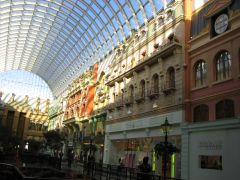
\includegraphics[width=.45\columnwidth]{Lorem}} \quad
\subfloat[Pan ma signo]
{\label{fig:example-b}%
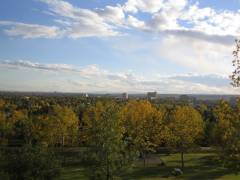
\includegraphics[width=.45\columnwidth]{Ipsum}} \\
\subfloat[Methodicamente o uno]
{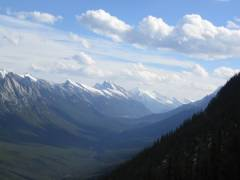
\includegraphics[width=.45\columnwidth]{Dolor}} \quad
\subfloat[Titulo debitas]
{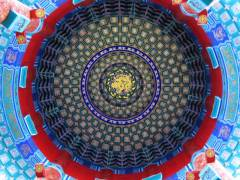
\includegraphics[width=.45\columnwidth]{Sit}}
\caption[Tu duo titulo debitas latente]{Tu duo titulo debitas latente}
\label{fig:example}
\end{figure}
Please note that the content of this section is just some dummy text. It isn't a real language.

Lorem ipsum dolor sit amet, consectetuer adipiscing elit. Ut purus elit, vestibulum ut, placerat ac, adipiscing vitae, felis. Curabitur dictum gravida mauris.

\subsection*{A subsection}

\lipsum[2]

\subsubsection*{A sub-subsection}

\lipsum[7]

\paragraph{A paragraph}
Lorem ipsum dolor sit amet, consectetuer adipiscing elit. Ut purus elit, vestibulum ut, placerat ac, adipiscing vitae, felis. Curabitur dictum gravida mauris. Nam arcu libero, nonummy eget, consectetuer id, vulputate a, magna.

\paragraph{Another paragraph}
Cras nec ante, pellentesque a nulla, cum sociis natoque penatibus et magnis dis parturient montes, nascetur ridiculus mus. Aliquam tincidunt urna

\bigskip

Donec aliquet, tortor sed accumsan bibendum, erat ligula aliquet magna, vitae ornare odio metus a mi. Morbi ac orci et nisl hendrerit mollis. Suspendisse ut massa. Cras nec ante. Pellentesque a nulla. Cum sociis natoque penatibus et magnis dis parturient montes, nascetur ridiculus mus. Aliquam tincidunt urna.

\begin{description}
\item[Mane] Lorem ipsum dolor sit amet, consectetuer adipiscing elit.
\item[Tekel] Ut purus elit, vestibulum ut, placerat ac, adipiscing vitae, felis. Curabitur dictum gravida mauris.
\item[Fares] Nam arcu libero, nonummy eget, consectetuer
id, vulputate a, magna.
\end{description}

\begin{table}
\caption{Lorem ipsum dolor sit amet}
\centering
\begin{tabular}{ll}
\toprule
\textbf{Alkaloid} & \textbf{Origin} \\
\midrule
atropine & belladonna \\
morphine & poppy \\
nicotine & tobacco \\
\bottomrule
\end{tabular}
\end{table}

Suspendisse vel felis. Ut lorem lorem, interdum eu, tincidunt sit amet, laoreet vitae, arcu. Aenean faucibus pede eu ante. Praesent enim elit, rutrum at, molestie non, nonummy vel, nisl. Ut lectus eros, malesuada sit amet, fermentum eu, sodales cursus, magna. Donec eu purus. Quisque vehicula, urna sed ultricies auctor, pede lorem egestas dui, et convallis elit erat sed nulla.

\subsection*{Some formulas}

Una formula in linea viene incorporata nel testo: $\lim_{n \to \infty}\sum_{k=1}^n \frac{1}{k^2} = \frac{\pi^2}{6}$, per esempio. Come si osserva, \LaTeX{} fa \emph{il possibile} per comprimerla e modificare il meno possibile l'interlinea nel capoverso che la contiene.
Una formula in display viene invece composta da \LaTeX{} su linee a parte, separate dal contesto con adeguati spazi bianchi per metterla in mostra e farla risaltare sulla pagina.
\begin{equation}
\lim_{n \to \infty}\sum_{k=1}^n \frac{1}{k^2}= \frac{\pi^2}{6}
\end{equation}
Come si osserva, ora la formula risulta centrata, non compressa, e tutti i suoi elementi occupano il giusto spazio con un risultato finale di grande respiro.

Integer tempus convallis augue. Etiam facilisis. Nunc elementum fermentum wisi. Aenean placerat. Ut imperdiet, enim sed gravida sollicitudin, felis odio placerat quam, ac pulvinar elit purus eget enim.

\begin{equation}
\int_a^{a+T}f(x)\,dx= \int_0^T f(x)\,dx
\qquad
\oint f(z)\,dz=2\pi i
\end{equation}

Nulla malesuada porttitor diam. Donec felis erat, congue non, volutpat at, tincidunt tristique, libero. Vivamus viverra fermentum felis. Donec non- ummy pellentesque ante.

\begin{equation}
f(x_1,\dots,x_n)=  \prod_{k=1}^n x_k
\qquad
\sum_{k=1}^n x_k^2=1
\qquad
\biggl(\sum_n x_n^2\biggr)^{1/2}
\end{equation}

\lipsum[2]

\begin{equation}
\begin{bmatrix}
a_{11} & \dots & a_{1n} \\
a_{21} & \dots & a_{2n} \\
\hdotsfor{3} \\
a_{n1} & \dots & a_{nn}
\end{bmatrix}
\end{equation}

\lipsum[4]

\begin{equation}
\lim_{x\to 0}
\frac{\sin x}{x}=1 \qquad
\lim_{n\to +\infty}f_n=\delta
\end{equation}

Fusce mauris. Vestibulum luctus nibh at lectus. Sed bibendum, nulla a faucibus semper, leo velit ultricies tellus, ac venenatis arcu wisi vel nisl. Vestibulum diam.

\begin{equation}
n!=
\begin{cases}
1       & \text{if $n=0$} \\
n(n-1)! & \text{if $n\ge 1$}
\end{cases}
\end{equation}

Ut lectus eros, malesuada sit amet, fermentum eu, sodales cursus, magna. Donec eu purus. Quisque vehicula, urna sed ultricies auctor, pede lorem egestas dui, et convallis elit erat sed nulla. Donec luctus. Curabitur et nunc. Aliquam dolor odio, commodo pretium, ultricies non, pharetra in, velit.

\begin{equation}
x_G=
\frac{\displaystyle
      \sum_{i=1}^n m_ix_i}
{\displaystyle\sum_{i=1}^n m_i}
\end{equation}

\lipsum[6]

\begin{equation}
\kappa =\frac{\xi}{E_{\textrm{max}}}
\qquad
E_{\textup{max}} =\frac{2 m_{\textup{e}} \beta^2\gamma^2 }{1 +2\gamma m_{\textup{e}}/m_{\textrm{x}} + ( m_{\textup{e}}/m_{\textup{x}})^2}
\end{equation}

\lipsum[8]
\end{comment}
% !TEX TS-program = pdflatex
% !TEX root = ../tesi.tex

%************************************************
\chapter{Genesis}
\label{chp:fundamentals}
%************************************************

This chapter introduces the main idea of my work. The role of this section is to connect the artistic concept of the work to the technical realization



\section{Gamification}

The concept of gamification is related to elements and dynamics belonging to the dimension of videogames used in non-ludic contexts. That's the application of video game creation principles to create an immersive experience for users involved in a non-ludic reality to increase their level of interaction with it.
The phenomenon of gamification takes place when the unconscious of a human being is influenced by actions and mechanisms belonging to a virtual dimension created by ourselves: the video games. This leads to the settle down, in the emotional depths of the player, of certain elements of the dimension of video games, which are then transported into ours by the user himself.
The concept of gamification took hold starting from the conference, held in February 2010 on the occasion of the "D.I.C.E. Summit" in Las Vegas, by game designer \textbf{Jesse Schell}
An experience that leads to looking at real world experiences as if we were in a video game so that they are particularly effective. The application to real-life game strategies.
Gamification is all of this.
In wich way the action performed in a videogame influence the behaviors that a person can have in real life? And, above all, wich are the dynamics that are brought into the real life? There are severals:

\begin{compactitem}
	\item Complete a level or a mission to get another one
	\item Exibith awards
	\item Accumulate points
	\item Get rewards and gifts
	\item Identify enemies
\end{compactitem}

How do I apply this concept to my own work? It create and manage an interactive composition exercise in order to immerse the user/gamer at the deepest level of complicity, up to making him both the user and composer of the performance at the same time. My work alows the player to make an electroacoustic performance by getting into the game, I've reached this goal by editing compositional gestures linked to the trigger of the events in the video game.
It's possible to influence and modify people's behaviour, favoring the emergence and consolidation of active interest on the part of the users involved in the essence of the game, whether this is related to the increase in emotional involvement on the part of the player or the influence that dynamics of the game can have on him.

\begin{figure}
	\begin{center}
		
\includegraphics[width=1\textwidth]{image9.jpg}
	\end{center}
\end{figure}

\section{interactive electroacoustic composition through the game}

The essence of the work is in the implementation of the audio: the sound design is made in an alternative way to the traditional one, creating sounds that interact with the player's gestures by abstraction rather than by causality: usually in a video game the actions performed correspond to sounds that have a link with the physics with which we are used to interact; this type of feedback requires that the sounds are generated by causality, following precise rules. In my work, the sounds are totally disconnected from the causality of the actions performed, creating a new abstract sound dimension
The events are denaturalized: they detach the gesture of the sound object from the reproduced sound.
It is a game of expectations: when the player made a gesture, electroacoustic sounds are generated which "normally" do not correspond to the sounds generated in a video game. Nervous and elusive impulses are therefore created by soft and dilated gestures, or sounds with a long attack and long decay time by simple and rapid gestures: the sounds and the music therefore does not satisfy the player's expectations, because they seem to respond to physical laws unknown to us, belonging to an alternative reality even to the virtual one.
In fact, the work is an interactive electroacoustic game that gives to the player the faculty of composer and player, without even being able to realize it.
In the following paragraphs I will describe the traditional workflow of a sound designer, talking about the differences from my compositional approach.

\begin{comment}
\begin{code}
\documentclass[\meta{\dots\unkern}]{scrreprt} % or scrbook or scrartcl

\usepackage[\meta{\dots\unkern}]{classicthesis}
\usepackage{arsclassica}

\begin{document}
\dots
\end{document}
\end{code}

For example, this document has been produced with the following code:
\begin{code}
\documentclass[a4paper,twoside,openright,titlepage,
               headinclude,footinclude,BCOR5mm,
               numbers=noenddot,cleardoublepage=empty,
               tablecaptionabove]{scrreprt}

\usepackage{\meta{\dots\unkern}}
\usepackage{subfig}
\usepackage[eulerchapternumbers,subfig,beramono,eulermath,pdfspacing]%
           {classicthesis}
\usepackage{arsclassica}

\begin{document}
\dots
\end{document}
\end{code}

It is recommended to use the \optname{beramono} and \optname{eulerchapternumbers} options together with \arsclassica.



\section{Style}

The typographical style achieved with \arsclassica{} differs from \classicthesis{} in the following points:
\begin{itemize}
\item use of Iwona font, by Janusz Nowacki, for the sectioning unit titles (chapters, sections, subsections, sub-subsections, paragraphs and subparagraphs), for the description list labels, the headlines and the caption labels (\classicthesis{} doesn't use any sans serif font);
\item customized chapter numbers;
\item semi-transparent headlines; the headlines are separated from the page number by a small rule;
\item caption labels in boldface (\classicthesis{} doesn't use any boldface font);
\item itemize lists with semi-transparent bullets.
\end{itemize}

\arsclassica{} is designed  to provide a ready-to-use typographical style: for this reason it has no loading options and it is \emph{not} configurable or customizable in any way. If you change the previous settings, you'll risk to destroy the balance of the style, so it is \emph{highly recommended} to keep them unchanged.

One of the principles of \LaTeX{} is that it allows the author to take no interest in the typographical questions, permitting him to focus only on the structure and the contents of his document. This fact should always be kept in mind: using a style written by others, the user accepts all the typographical settings chosen for him by the author of the style, and he isn't forced to study typography to fine-tune the layout of his publications. This is the case of \arsclassica{} too: if you change its settings, you'll deny this philosophy and, consequently, you'll have to study (a lot of) typography to achieve acceptable results.

The style achieved with \arsclassica{} is \emph{not} therefore configurable or customizable. The typographical style is very personal: if you like this package and find attractive the idea to take no interest in the problem of the style definition, then you'll use \arsclassica{} with satisfaction; otherwise, if you have different needs or you aren't satisfied with the layout of the package, then you should try other classes or packages, even building your own style.



\section{Important}

To write a document according to the \arsclassica{} style, you have to follow some very simple rules.
\begin{itemize}
\item Don't change \emph{for any reason} the \arsclassica{} settings (fonts, text body size, colors, \dots).
\item The sectioning unit titles (chapters, section, subsections, \dots) have to be \emph{one line long}, possibly in \emph{plain text} (no symbols, formulas or code fragments). If you have titles longer than one line, try and rephrase them: you can almost always do it.
\item In the table of contents and in the list of tables and figures, captions have to be \emph{one line long}, possibly in \emph{plain text}. Use the optional argument of sectioning commands and of \cmdname{caption}, if necessary.
\item Don't use \optname{tocaligned} and \optname{dottedtoc} options of \classicthesis: the default table of contents does the job very well (see the documentation of \classicthesis{} for a nice discussion of this point).
\item Don't use vertical or double rules in your tables (see the documentation of \pkgname{booktabs}).
\item Use footnotes and margin notes very sparingly.
\item If your document includes graphs and plots, draw them using \LaTeX{} (by \pkgname{Ti\emph{k}Z} and \pkgname{pgfplots}, for example) and not an external software. This is the only way to get the best typographical outcome.
\end{itemize}



\section{Examples}

\begin{figure}
\centering
\subfloat[Asia personas duo]
{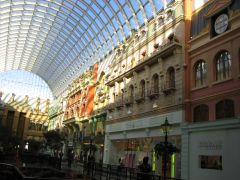
\includegraphics[width=.45\columnwidth]{Lorem}} \quad
\subfloat[Pan ma signo]
{\label{fig:example-b}%
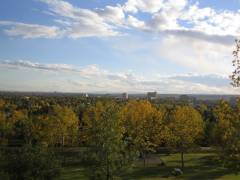
\includegraphics[width=.45\columnwidth]{Ipsum}} \\
\subfloat[Methodicamente o uno]
{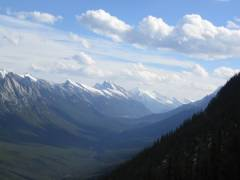
\includegraphics[width=.45\columnwidth]{Dolor}} \quad
\subfloat[Titulo debitas]
{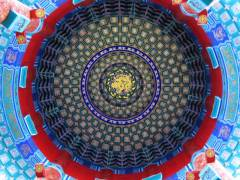
\includegraphics[width=.45\columnwidth]{Sit}}
\caption[Tu duo titulo debitas latente]{Tu duo titulo debitas latente}
\label{fig:example}
\end{figure}

Please note that the content of this section is just some dummy text. It isn't a real language.

Lorem ipsum dolor sit amet, consectetuer adipiscing elit. Ut purus elit, vestibulum ut, placerat ac, adipiscing vitae, felis. Curabitur dictum gravida mauris.

\subsection*{A subsection}

\lipsum[2]

\subsubsection*{A sub-subsection}

\lipsum[7]

\paragraph{A paragraph}
Lorem ipsum dolor sit amet, consectetuer adipiscing elit. Ut purus elit, vestibulum ut, placerat ac, adipiscing vitae, felis. Curabitur dictum gravida mauris. Nam arcu libero, nonummy eget, consectetuer id, vulputate a, magna.

\paragraph{Another paragraph}
Cras nec ante, pellentesque a nulla, cum sociis natoque penatibus et magnis dis parturient montes, nascetur ridiculus mus. Aliquam tincidunt urna

\bigskip

Donec aliquet, tortor sed accumsan bibendum, erat ligula aliquet magna, vitae ornare odio metus a mi. Morbi ac orci et nisl hendrerit mollis. Suspendisse ut massa. Cras nec ante. Pellentesque a nulla. Cum sociis natoque penatibus et magnis dis parturient montes, nascetur ridiculus mus. Aliquam tincidunt urna.

\begin{description}
\item[Mane] Lorem ipsum dolor sit amet, consectetuer adipiscing elit.
\item[Tekel] Ut purus elit, vestibulum ut, placerat ac, adipiscing vitae, felis. Curabitur dictum gravida mauris.
\item[Fares] Nam arcu libero, nonummy eget, consectetuer
id, vulputate a, magna.
\end{description}

\begin{table}
\caption{Lorem ipsum dolor sit amet}
\centering
\begin{tabular}{ll}
\toprule
\textbf{Alkaloid} & \textbf{Origin} \\
\midrule
atropine & belladonna \\
morphine & poppy \\
nicotine & tobacco \\
\bottomrule
\end{tabular}
\end{table}

Suspendisse vel felis. Ut lorem lorem, interdum eu, tincidunt sit amet, laoreet vitae, arcu. Aenean faucibus pede eu ante. Praesent enim elit, rutrum at, molestie non, nonummy vel, nisl. Ut lectus eros, malesuada sit amet, fermentum eu, sodales cursus, magna. Donec eu purus. Quisque vehicula, urna sed ultricies auctor, pede lorem egestas dui, et convallis elit erat sed nulla.

\subsection*{Some formulas}

Una formula in linea viene incorporata nel testo: $\lim_{n \to \infty}\sum_{k=1}^n \frac{1}{k^2} = \frac{\pi^2}{6}$, per esempio. Come si osserva, \LaTeX{} fa \emph{il possibile} per comprimerla e modificare il meno possibile l'interlinea nel capoverso che la contiene.
Una formula in display viene invece composta da \LaTeX{} su linee a parte, separate dal contesto con adeguati spazi bianchi per metterla in mostra e farla risaltare sulla pagina.
\begin{equation}
\lim_{n \to \infty}\sum_{k=1}^n \frac{1}{k^2}= \frac{\pi^2}{6}
\end{equation}
Come si osserva, ora la formula risulta centrata, non compressa, e tutti i suoi elementi occupano il giusto spazio con un risultato finale di grande respiro.

Integer tempus convallis augue. Etiam facilisis. Nunc elementum fermentum wisi. Aenean placerat. Ut imperdiet, enim sed gravida sollicitudin, felis odio placerat quam, ac pulvinar elit purus eget enim.

\begin{equation}
\int_a^{a+T}f(x)\,dx= \int_0^T f(x)\,dx
\qquad
\oint f(z)\,dz=2\pi i
\end{equation}

Nulla malesuada porttitor diam. Donec felis erat, congue non, volutpat at, tincidunt tristique, libero. Vivamus viverra fermentum felis. Donec non- ummy pellentesque ante.

\begin{equation}
f(x_1,\dots,x_n)=  \prod_{k=1}^n x_k
\qquad
\sum_{k=1}^n x_k^2=1
\qquad
\biggl(\sum_n x_n^2\biggr)^{1/2}
\end{equation}

\lipsum[2]

\begin{equation}
\begin{bmatrix}
a_{11} & \dots & a_{1n} \\
a_{21} & \dots & a_{2n} \\
\hdotsfor{3} \\
a_{n1} & \dots & a_{nn}
\end{bmatrix}
\end{equation}

\lipsum[4]

\begin{equation}
\lim_{x\to 0}
\frac{\sin x}{x}=1 \qquad
\lim_{n\to +\infty}f_n=\delta
\end{equation}

Fusce mauris. Vestibulum luctus nibh at lectus. Sed bibendum, nulla a faucibus semper, leo velit ultricies tellus, ac venenatis arcu wisi vel nisl. Vestibulum diam.

\begin{equation}
n!=
\begin{cases}
1       & \text{if $n=0$} \\
n(n-1)! & \text{if $n\ge 1$}
\end{cases}
\end{equation}

Ut lectus eros, malesuada sit amet, fermentum eu, sodales cursus, magna. Donec eu purus. Quisque vehicula, urna sed ultricies auctor, pede lorem egestas dui, et convallis elit erat sed nulla. Donec luctus. Curabitur et nunc. Aliquam dolor odio, commodo pretium, ultricies non, pharetra in, velit.

\begin{equation}
x_G=
\frac{\displaystyle
      \sum_{i=1}^n m_ix_i}
{\displaystyle\sum_{i=1}^n m_i}
\end{equation}

\lipsum[6]

\begin{equation}
\kappa =\frac{\xi}{E_{\textrm{max}}}
\qquad
E_{\textup{max}} =\frac{2 m_{\textup{e}} \beta^2\gamma^2 }{1 +2\gamma m_{\textup{e}}/m_{\textrm{x}} + ( m_{\textup{e}}/m_{\textup{x}})^2}
\end{equation}

\lipsum[8]
\end{comment}
% !TEX TS-program = pdflatex
% !TEX root = ../tesi.tex

%************************************************
\chapter{Sound design workflow}
\label{chp:intro}
%************************************************

Although is complex to predict the actions of a video game, is possible to control the player's emotions as we want, all this is made possible only by music: the primordial language that regulates the emotional genesis of each person.
There are, obviously, several parameters for making an overall evaluation of the audio implementation for a video game, which concerns both the form and the accuracy of the sounds.
But the parameter of evaluation changes when changing the type and the style of the game too.
The composer and sound designer Brian Schmidt, who worked on tons of games such as NARC, talking about the audio implementation for Arcade games, said:
\begin{flushright}
	\itshape
	Althought games were short, they'd often have a lot of different modes or mini-game \\
	within them, each requiring their own music. \\
	So even a simple painball machine game would have a good 25-30 minutes of interactive original score\\
	\medskip
	--- Brian Schmidt
\end{flushright}

Just as, as far as can be deduced from his words, arcade games have their specific needs for sound design and music composition, in the same way, every different type of video game has its specific needs, let's talk about some of these:

	\paragraph{Scrolling} This type is identified in video games that go in one direction, without level or scene changing. Typically, the sound design is easier, because in just one scene the materials and the actions are ever the same. Isn't the same for the music composition: in this type of videogame the music has to change continuously depending on some element, such as the number of enemies, the level of the health of the main character, the fighting moment, and something else. the main sub-genre of this type of games are:

		\begin{compactitem}
			\item Maze-Chase Games, such as Pac-Man(1982). A game in wich the main character navigate through a maze
			\item Platform games, such as Donkey Kong(1981). A game in wich the main character jump or move from platform to platform
			\item Shot'em Ups, such as Centipede(1981). In wich the main character have a gun to kill every enemy
		\end{compactitem}

	\begin{figure}[h]
		\begin{center}
			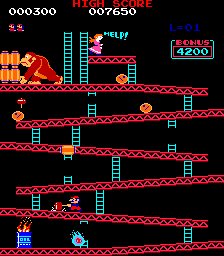
\includegraphics[width=.8\textwidth]{DK.png}
			\caption{the Scrolling Platform game Donkey Kong (1981)}
		\end{center}
	\end{figure}

	\paragraph{Games with levels} Have different needs. The music must change for each scene, as well as the character of the sound design based on the materials used and the soundscape of the scene: a noisy bar, a quiet forest, and an empty room. Each of these environments generates different soundscapes that sound design must adapt to.

The video-game chosen for this implementation is a \textbf{level based game} in first person. Now let's talk about the main elements of an accurate sound design for this type of game.

\section{Polishing}

A player's actions move a video game in one direction rather than another. Is essential to provide feedback to the player based on the importance of the action performed. Music and sounds are essential to guide the player to make choices within the video game. Polishing is an integral part of the ability to capture and immerse the player in the virtual dimension of the game. The dynamics of sound play a fundamental role in this: a good sound designer must be able, through gain staging, to capture the player's attention on the actions performed
In the implementation of this work, that's an alternative approach in the parameter of polishing: There isn't a great work of gain staging, but on the character of the sounds: the more a musical gesture is detached from the traditional idea of ​​sound design, the greater the player's involvement will be. It's a game of expectations: therefore I worked more by abstraction than by causality when I needed to bring the player's attention through an action

\section{Mix}
The balance of frequencies in the sound design image is another important item. Its main goals are 2:

\begin{itemize}
	\item To balance the timbre of the overall audio
	\item To prepare the player's ear for twists and turns
\end{itemize}

Mixing sounds to give roles to each of them in the frequency spectrum best distributes sound energy.
As already mentioned, the durations of the musical gestures are deliberately prolonged and dispersive compared to a traditional approach. This factor certainly doesn't respect the idea of ​​giving a "role" to each sound. However, the material is equalized to maintain at least the "timbral" role of each sound.

\section{Levels of action}
For a sound designer, is useful to find order: spectrally and dynamically distinguish the sounds belonging to the different levels of action: background, actions, and events.

\paragraph{Background sound} are identified in the soundscape. For example, if the main scene is a forest, the background sounds will be the birds, the wind, or the leaves. Despite in this work there isn't a great distinction in the gesture of the implementation, is respected a simple hierarchy structure, giving the role of "background" sounds to the music carpet: an electroacoustic simple immersive flow of many types of timbres.

\paragraph{Actions sound} are related to the direction of the main character: footsteps, pick-up objects, etc. In this implementation, these are the closest sounds to those of a traditional sound design. Not so much for the timbre of the sounds as for their duration, because, since there are short and continuous actions, I couldn't have associated complex musical gestures with them: I need simple and short sounds that are not repetitive, even though they repeat themselves continuously. So I opted for classic electroacoustic glitch sounds, applying random modulations on different parameters (such as volume, pitch, LowPass, and HighPass filter, etc) and inserting them in a random container. In this way, they will always sound different, even though the sounds used for these gestures, such as footsteps, for example, are only 3
\paragraph{Events sounds} are the most important for the involving of the player in the game. For these reason, in this implementation, these sound are the loudest. In the most chase, they are short and loud impulses.

\section{differences between the implementation of sound for game and movies}
The main difference between implementing audio for games and movies is the linearity: a movie has its timeline in which events are located. A film sound designer or composer knows the order of the events and when each one begins and ends, so he has a timeline to follow for adding sounds, gestures, and music in a specific order. A game sound designer must be able to make short and functional gestures, trying to predict which sounds will overlap. Every sound and every music theme must be able to fit with another one, because after a battle scene for example, anything could happen, distorting the mood of the context, precisely because of the non-linearity of the events.

\begin{comment}\begin{code}
\documentclass[\meta{\dots\unkern}]{scrreprt} % or scrbook or scrartcl

\usepackage[\meta{\dots\unkern}]{classicthesis}
\usepackage{arsclassica}

\begin{document}
\dots
\end{document}
\end{code}

For example, this document has been produced with the following code:
\begin{code}
\documentclass[a4paper,twoside,openright,titlepage,
               headinclude,footinclude,BCOR5mm,
               numbers=noenddot,cleardoublepage=empty,
               tablecaptionabove]{scrreprt}

\usepackage{\meta{\dots\unkern}}
\usepackage{subfig}
\usepackage[eulerchapternumbers,subfig,beramono,eulermath,pdfspacing]%
           {classicthesis}
\usepackage{arsclassica}

\begin{document}
\dots
\end{document}
\end{code}

It is recommended to use the \optname{beramono} and \optname{eulerchapternumbers} options together with \arsclassica.



\section{Style}

The typographical style achieved with \arsclassica{} differs from \classicthesis{} in the following points:
\begin{itemize}
\item use of Iwona font, by Janusz Nowacki, for the sectioning unit titles (chapters, sections, subsections, sub-subsections, paragraphs and subparagraphs), for the description list labels, the headlines and the caption labels (\classicthesis{} doesn't use any sans serif font);
\item customized chapter numbers;
\item semi-transparent headlines; the headlines are separated from the page number by a small rule;
\item caption labels in boldface (\classicthesis{} doesn't use any boldface font);
\item itemize lists with semi-transparent bullets.
\end{itemize}

\arsclassica{} is designed  to provide a ready-to-use typographical style: for this reason it has no loading options and it is \emph{not} configurable or customizable in any way. If you change the previous settings, you'll risk to destroy the balance of the style, so it is \emph{highly recommended} to keep them unchanged.

One of the principles of \LaTeX{} is that it allows the author to take no interest in the typographical questions, permitting him to focus only on the structure and the contents of his document. This fact should always be kept in mind: using a style written by others, the user accepts all the typographical settings chosen for him by the author of the style, and he isn't forced to study typography to fine-tune the layout of his publications. This is the case of \arsclassica{} too: if you change its settings, you'll deny this philosophy and, consequently, you'll have to study (a lot of) typography to achieve acceptable results.

The style achieved with \arsclassica{} is \emph{not} therefore configurable or customizable. The typographical style is very personal: if you like this package and find attractive the idea to take no interest in the problem of the style definition, then you'll use \arsclassica{} with satisfaction; otherwise, if you have different needs or you aren't satisfied with the layout of the package, then you should try other classes or packages, even building your own style.



\section{Important}

To write a document according to the \arsclassica{} style, you have to follow some very simple rules.
\begin{itemize}
\item Don't change \emph{for any reason} the \arsclassica{} settings (fonts, text body size, colors, \dots).
\item The sectioning unit titles (chapters, section, subsections, \dots) have to be \emph{one line long}, possibly in \emph{plain text} (no symbols, formulas or code fragments). If you have titles longer than one line, try and rephrase them: you can almost always do it.
\item In the table of contents and in the list of tables and figures, captions have to be \emph{one line long}, possibly in \emph{plain text}. Use the optional argument of sectioning commands and of \cmdname{caption}, if necessary.
\item Don't use \optname{tocaligned} and \optname{dottedtoc} options of \classicthesis: the default table of contents does the job very well (see the documentation of \classicthesis{} for a nice discussion of this point).
\item Don't use vertical or double rules in your tables (see the documentation of \pkgname{booktabs}).
\item Use footnotes and margin notes very sparingly.
\item If your document includes graphs and plots, draw them using \LaTeX{} (by \pkgname{Ti\emph{k}Z} and \pkgname{pgfplots}, for example) and not an external software. This is the only way to get the best typographical outcome.
\end{itemize}



%\section{Examples}
%intendo sostituire queste immagini con qualcuna inerente al mio progetto
\begin{figure}
\centering
\subfloat[Asia personas duo]
{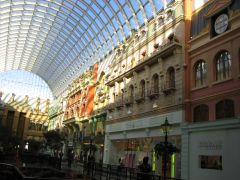
\includegraphics[width=.45\columnwidth]{Lorem}} \quad
\subfloat[Pan ma signo]
{\label{fig:example-b}%
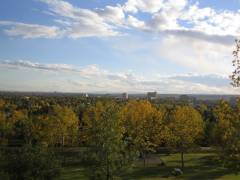
\includegraphics[width=.45\columnwidth]{Ipsum}} \\
\subfloat[Methodicamente o uno]
{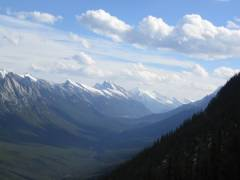
\includegraphics[width=.45\columnwidth]{Dolor}} \quad
\subfloat[Titulo debitas]
{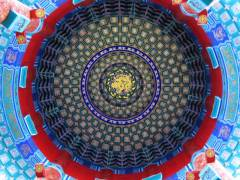
\includegraphics[width=.45\columnwidth]{Sit}}
\caption[Tu duo titulo debitas latente]{Tu duo titulo debitas latente}
\label{fig:example}
\end{figure}
Please note that the content of this section is just some dummy text. It isn't a real language.

Lorem ipsum dolor sit amet, consectetuer adipiscing elit. Ut purus elit, vestibulum ut, placerat ac, adipiscing vitae, felis. Curabitur dictum gravida mauris.

\subsection*{A subsection}

\lipsum[2]

\subsubsection*{A sub-subsection}

\lipsum[7]

\paragraph{A paragraph}
Lorem ipsum dolor sit amet, consectetuer adipiscing elit. Ut purus elit, vestibulum ut, placerat ac, adipiscing vitae, felis. Curabitur dictum gravida mauris. Nam arcu libero, nonummy eget, consectetuer id, vulputate a, magna.

\paragraph{Another paragraph}
Cras nec ante, pellentesque a nulla, cum sociis natoque penatibus et magnis dis parturient montes, nascetur ridiculus mus. Aliquam tincidunt urna

\bigskip

Donec aliquet, tortor sed accumsan bibendum, erat ligula aliquet magna, vitae ornare odio metus a mi. Morbi ac orci et nisl hendrerit mollis. Suspendisse ut massa. Cras nec ante. Pellentesque a nulla. Cum sociis natoque penatibus et magnis dis parturient montes, nascetur ridiculus mus. Aliquam tincidunt urna.

\begin{description}
\item[Mane] Lorem ipsum dolor sit amet, consectetuer adipiscing elit.
\item[Tekel] Ut purus elit, vestibulum ut, placerat ac, adipiscing vitae, felis. Curabitur dictum gravida mauris.
\item[Fares] Nam arcu libero, nonummy eget, consectetuer
id, vulputate a, magna.
\end{description}

\begin{table}
\caption{Lorem ipsum dolor sit amet}
\centering
\begin{tabular}{ll}
\toprule
\textbf{Alkaloid} & \textbf{Origin} \\
\midrule
atropine & belladonna \\
morphine & poppy \\
nicotine & tobacco \\
\bottomrule
\end{tabular}
\end{table}

Suspendisse vel felis. Ut lorem lorem, interdum eu, tincidunt sit amet, laoreet vitae, arcu. Aenean faucibus pede eu ante. Praesent enim elit, rutrum at, molestie non, nonummy vel, nisl. Ut lectus eros, malesuada sit amet, fermentum eu, sodales cursus, magna. Donec eu purus. Quisque vehicula, urna sed ultricies auctor, pede lorem egestas dui, et convallis elit erat sed nulla.

\subsection*{Some formulas}

Una formula in linea viene incorporata nel testo: $\lim_{n \to \infty}\sum_{k=1}^n \frac{1}{k^2} = \frac{\pi^2}{6}$, per esempio. Come si osserva, \LaTeX{} fa \emph{il possibile} per comprimerla e modificare il meno possibile l'interlinea nel capoverso che la contiene.
Una formula in display viene invece composta da \LaTeX{} su linee a parte, separate dal contesto con adeguati spazi bianchi per metterla in mostra e farla risaltare sulla pagina.
\begin{equation}
\lim_{n \to \infty}\sum_{k=1}^n \frac{1}{k^2}= \frac{\pi^2}{6}
\end{equation}
Come si osserva, ora la formula risulta centrata, non compressa, e tutti i suoi elementi occupano il giusto spazio con un risultato finale di grande respiro.

Integer tempus convallis augue. Etiam facilisis. Nunc elementum fermentum wisi. Aenean placerat. Ut imperdiet, enim sed gravida sollicitudin, felis odio placerat quam, ac pulvinar elit purus eget enim.

\begin{equation}
\int_a^{a+T}f(x)\,dx= \int_0^T f(x)\,dx
\qquad
\oint f(z)\,dz=2\pi i
\end{equation}

Nulla malesuada porttitor diam. Donec felis erat, congue non, volutpat at, tincidunt tristique, libero. Vivamus viverra fermentum felis. Donec non- ummy pellentesque ante.

\begin{equation}
f(x_1,\dots,x_n)=  \prod_{k=1}^n x_k
\qquad
\sum_{k=1}^n x_k^2=1
\qquad
\biggl(\sum_n x_n^2\biggr)^{1/2}
\end{equation}

\lipsum[2]

\begin{equation}
\begin{bmatrix}
a_{11} & \dots & a_{1n} \\
a_{21} & \dots & a_{2n} \\
\hdotsfor{3} \\
a_{n1} & \dots & a_{nn}
\end{bmatrix}
\end{equation}

\lipsum[4]

\begin{equation}
\lim_{x\to 0}
\frac{\sin x}{x}=1 \qquad
\lim_{n\to +\infty}f_n=\delta
\end{equation}

Fusce mauris. Vestibulum luctus nibh at lectus. Sed bibendum, nulla a faucibus semper, leo velit ultricies tellus, ac venenatis arcu wisi vel nisl. Vestibulum diam.

\begin{equation}
n!=
\begin{cases}
1       & \text{if $n=0$} \\
n(n-1)! & \text{if $n\ge 1$}
\end{cases}
\end{equation}

Ut lectus eros, malesuada sit amet, fermentum eu, sodales cursus, magna. Donec eu purus. Quisque vehicula, urna sed ultricies auctor, pede lorem egestas dui, et convallis elit erat sed nulla. Donec luctus. Curabitur et nunc. Aliquam dolor odio, commodo pretium, ultricies non, pharetra in, velit.

\begin{equation}
x_G=
\frac{\displaystyle
      \sum_{i=1}^n m_ix_i}
{\displaystyle\sum_{i=1}^n m_i}
\end{equation}

\lipsum[6]

\begin{equation}
\kappa =\frac{\xi}{E_{\textrm{max}}}
\qquad
E_{\textup{max}} =\frac{2 m_{\textup{e}} \beta^2\gamma^2 }{1 +2\gamma m_{\textup{e}}/m_{\textrm{x}} + ( m_{\textup{e}}/m_{\textup{x}})^2}
\end{equation}

\lipsum[8]
\end{comment}

% !TEX TS-program = pdflatex
% !TEX root = ../tesi.tex

%************************************************
\chapter{My implementation}
\label{chp:fundamentals}
%************************************************

My main work in on audio implementation: i chose to use an open-source game written in C++ called Cube,
Cube is an 2D low-poly retro-style video-game with a low graphic resolution whose source code is available online. The definitions "low-poly" and "retro-style" are common used to describe the style of the graphic, witch is based on different scenes realized with "low-poly" objects, which are graphic components formed by a few geometric figures, which gives them an "angular" appearance. The "retro-style" is a type of graphic style recalls the graphics of the video games of the 80s and 90s, when the pixels were more visible and the resolution of the displays was much lower than the current one.
I chose to work on the sound design for Cube because the game is very simple, which allowed me to do a job faithful to my compositional intentions. In addition, this game was written for educational purposes: therefore, in addition to making the audio implementation intuitive, the source code is compatible with the most common audio implementation engines for video games. These softwares are called "middleware", and there are several:

\begin{itemsize}
	\item Wwise: the middleware i chose to use because is the most common and popular in the game-audio industry
	\item Fabric: An audio middleware developed by Tazman-Audio
	\item Elias: An audio middleware that uses A.I.
\end{itemsize}



\section{Middleware}
\begin{flushright}
	\itshape
	Why was middleware needed? Well, music and sound designers and programmers developed middleware \\
	so that the designers and composer could gain more control over how their audio was used in games.\\
	Middleware is based on the idea that the video game is an interactive medium, \\
	so all audio elements within the game should be interactive as well. \\
	\medskip
	--- Steve Horowitz and Scott Looney, "The essential guide to game audio "
\end{flushright}

Middlewares are softwares that sits between the game engine and the audio engine, providing a set of tools and features to manage audio content and processing. Middleware typically provides a layer of abstraction between the game engine and the audio engine.
Middleware can perform a variety of tasks, such as audio playback, dynamic mixing, audio processing, sound effects, and music management. It can also handle the integration of external audio tools and libraries, such as plug-ins. For example, Wwise can communicate with Steinberg Nuendo. In Wwise can be also loaded the plug-ins produced by Izotope for audio processing can be integrated
When a game is being developed, the middleware receives audio data from the game engine, processes it according to the developer's settings, and sends the soundbanks to the audio engine for playback.
A Soundbank is a collection of audio files, that are packaged together into a single file for efficient loading and playback during the game.
Sound banks typically contain metadata that describes how the audio files should be played back in the game, such as volume, panning, and spatial positioning information. Sound banks are usually created using middleware tools and are loaded by the game engine during runtime. By using sound banks, is possible to enabling a more immersive and dynamic audio experience in the game.

% devo aggiungere testo su cos'è e come funziona Wwise(soundbanks, eventi etc)

\section{Random controllers}
Some of these events are grouped in differents containers. The containers are variations of the calling action of the differents events witch can trigger the sounds of the events in so many different ways, one of these is called Random Container: a set of audio events that are recalled randomly at each trigger. used for example for footsteps or jump sounds
Is also possible to control randomically some values through the game parameters.
Game Parameters in Wwise are numeric variables that can be used to control audio behavior during application interaction. They are dynamic parameters that allow you to adjust different sound aspects in real time, such as volume, panning, transitions and more. Game Parameters offer a flexible way to create responsive and personalized audio interactions, also in randomic way. Is possible give to a game parameters a range of values ​​in which to recall a parameter at each trigger, such as the volume, for example in a range from -12 and -3dB, or the cutoff frequency of a lowpass filter, for example from 200 to 1000 Hz.

\section{Dynamic controllers}
Some of these events are modulated by RTPC (Real-Time Parameter Control). It's a system that allows you to control the sound parameters in real time while playing the game.
RTPC allows to change the values ​​of a parameter, such as the volume, the pitch or the cutoff frequency of a filter, dynamically and based on events or situations that appeares in the game. For example, RTPC could be used to increase the volume of the sound when the player approaches a noise source, or to increase the pitch (so the playback speed) of the heartbeat sound based on the ammount of the healt of the character. In this way, a more immersive and realistic sound experience can be created for the player.

\begin{comment}
\begin{code}
\documentclass[\meta{\dots\unkern}]{scrreprt} % or scrbook or scrartcl

\usepackage[\meta{\dots\unkern}]{classicthesis}
\usepackage{arsclassica}

\begin{document}
\dots
\end{document}
\end{code}

For example, this document has been produced with the following code:
\begin{code}
\documentclass[a4paper,twoside,openright,titlepage,
               headinclude,footinclude,BCOR5mm,
               numbers=noenddot,cleardoublepage=empty,
               tablecaptionabove]{scrreprt}

\usepackage{\meta{\dots\unkern}}
\usepackage{subfig}
\usepackage[eulerchapternumbers,subfig,beramono,eulermath,pdfspacing]%
           {classicthesis}
\usepackage{arsclassica}

\begin{document}
\dots
\end{document}
\end{code}

It is recommended to use the \optname{beramono} and \optname{eulerchapternumbers} options together with \arsclassica.



\section{Style}

The typographical style achieved with \arsclassica{} differs from \classicthesis{} in the following points:
\begin{itemize}
\item use of Iwona font, by Janusz Nowacki, for the sectioning unit titles (chapters, sections, subsections, sub-subsections, paragraphs and subparagraphs), for the description list labels, the headlines and the caption labels (\classicthesis{} doesn't use any sans serif font);
\item customized chapter numbers;
\item semi-transparent headlines; the headlines are separated from the page number by a small rule;
\item caption labels in boldface (\classicthesis{} doesn't use any boldface font);
\item itemize lists with semi-transparent bullets.
\end{itemize}

\arsclassica{} is designed  to provide a ready-to-use typographical style: for this reason it has no loading options and it is \emph{not} configurable or customizable in any way. If you change the previous settings, you'll risk to destroy the balance of the style, so it is \emph{highly recommended} to keep them unchanged.

One of the principles of \LaTeX{} is that it allows the author to take no interest in the typographical questions, permitting him to focus only on the structure and the contents of his document. This fact should always be kept in mind: using a style written by others, the user accepts all the typographical settings chosen for him by the author of the style, and he isn't forced to study typography to fine-tune the layout of his publications. This is the case of \arsclassica{} too: if you change its settings, you'll deny this philosophy and, consequently, you'll have to study (a lot of) typography to achieve acceptable results.

The style achieved with \arsclassica{} is \emph{not} therefore configurable or customizable. The typographical style is very personal: if you like this package and find attractive the idea to take no interest in the problem of the style definition, then you'll use \arsclassica{} with satisfaction; otherwise, if you have different needs or you aren't satisfied with the layout of the package, then you should try other classes or packages, even building your own style.



\section{Important}

To write a document according to the \arsclassica{} style, you have to follow some very simple rules.
\begin{itemize}
\item Don't change \emph{for any reason} the \arsclassica{} settings (fonts, text body size, colors, \dots).
\item The sectioning unit titles (chapters, section, subsections, \dots) have to be \emph{one line long}, possibly in \emph{plain text} (no symbols, formulas or code fragments). If you have titles longer than one line, try and rephrase them: you can almost always do it.
\item In the table of contents and in the list of tables and figures, captions have to be \emph{one line long}, possibly in \emph{plain text}. Use the optional argument of sectioning commands and of \cmdname{caption}, if necessary.
\item Don't use \optname{tocaligned} and \optname{dottedtoc} options of \classicthesis: the default table of contents does the job very well (see the documentation of \classicthesis{} for a nice discussion of this point).
\item Don't use vertical or double rules in your tables (see the documentation of \pkgname{booktabs}).
\item Use footnotes and margin notes very sparingly.
\item If your document includes graphs and plots, draw them using \LaTeX{} (by \pkgname{Ti\emph{k}Z} and \pkgname{pgfplots}, for example) and not an external software. This is the only way to get the best typographical outcome.
\end{itemize}



\section{Examples}

\begin{figure}
\centering
\subfloat[Asia personas duo]
{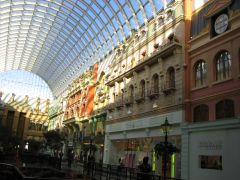
\includegraphics[width=.45\columnwidth]{Lorem}} \quad
\subfloat[Pan ma signo]
{\label{fig:example-b}%
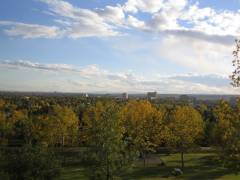
\includegraphics[width=.45\columnwidth]{Ipsum}} \\
\subfloat[Methodicamente o uno]
{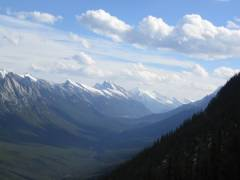
\includegraphics[width=.45\columnwidth]{Dolor}} \quad
\subfloat[Titulo debitas]
{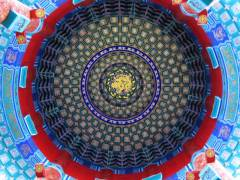
\includegraphics[width=.45\columnwidth]{Sit}}
\caption[Tu duo titulo debitas latente]{Tu duo titulo debitas latente}
\label{fig:example}
\end{figure}

Please note that the content of this section is just some dummy text. It isn't a real language.

Lorem ipsum dolor sit amet, consectetuer adipiscing elit. Ut purus elit, vestibulum ut, placerat ac, adipiscing vitae, felis. Curabitur dictum gravida mauris.

\subsection*{A subsection}

\lipsum[2]

\subsubsection*{A sub-subsection}

\lipsum[7]

\paragraph{A paragraph}
Lorem ipsum dolor sit amet, consectetuer adipiscing elit. Ut purus elit, vestibulum ut, placerat ac, adipiscing vitae, felis. Curabitur dictum gravida mauris. Nam arcu libero, nonummy eget, consectetuer id, vulputate a, magna.

\paragraph{Another paragraph}
Cras nec ante, pellentesque a nulla, cum sociis natoque penatibus et magnis dis parturient montes, nascetur ridiculus mus. Aliquam tincidunt urna

\bigskip

Donec aliquet, tortor sed accumsan bibendum, erat ligula aliquet magna, vitae ornare odio metus a mi. Morbi ac orci et nisl hendrerit mollis. Suspendisse ut massa. Cras nec ante. Pellentesque a nulla. Cum sociis natoque penatibus et magnis dis parturient montes, nascetur ridiculus mus. Aliquam tincidunt urna.

\begin{description}
\item[Mane] Lorem ipsum dolor sit amet, consectetuer adipiscing elit.
\item[Tekel] Ut purus elit, vestibulum ut, placerat ac, adipiscing vitae, felis. Curabitur dictum gravida mauris.
\item[Fares] Nam arcu libero, nonummy eget, consectetuer
id, vulputate a, magna.
\end{description}

\begin{table}
\caption{Lorem ipsum dolor sit amet}
\centering
\begin{tabular}{ll}
\toprule
\textbf{Alkaloid} & \textbf{Origin} \\
\midrule
atropine & belladonna \\
morphine & poppy \\
nicotine & tobacco \\
\bottomrule
\end{tabular}
\end{table}

Suspendisse vel felis. Ut lorem lorem, interdum eu, tincidunt sit amet, laoreet vitae, arcu. Aenean faucibus pede eu ante. Praesent enim elit, rutrum at, molestie non, nonummy vel, nisl. Ut lectus eros, malesuada sit amet, fermentum eu, sodales cursus, magna. Donec eu purus. Quisque vehicula, urna sed ultricies auctor, pede lorem egestas dui, et convallis elit erat sed nulla.

\subsection*{Some formulas}

Una formula in linea viene incorporata nel testo: $\lim_{n \to \infty}\sum_{k=1}^n \frac{1}{k^2} = \frac{\pi^2}{6}$, per esempio. Come si osserva, \LaTeX{} fa \emph{il possibile} per comprimerla e modificare il meno possibile l'interlinea nel capoverso che la contiene.
Una formula in display viene invece composta da \LaTeX{} su linee a parte, separate dal contesto con adeguati spazi bianchi per metterla in mostra e farla risaltare sulla pagina.
\begin{equation}
\lim_{n \to \infty}\sum_{k=1}^n \frac{1}{k^2}= \frac{\pi^2}{6}
\end{equation}
Come si osserva, ora la formula risulta centrata, non compressa, e tutti i suoi elementi occupano il giusto spazio con un risultato finale di grande respiro.

Integer tempus convallis augue. Etiam facilisis. Nunc elementum fermentum wisi. Aenean placerat. Ut imperdiet, enim sed gravida sollicitudin, felis odio placerat quam, ac pulvinar elit purus eget enim.

\begin{equation}
\int_a^{a+T}f(x)\,dx= \int_0^T f(x)\,dx
\qquad
\oint f(z)\,dz=2\pi i
\end{equation}

Nulla malesuada porttitor diam. Donec felis erat, congue non, volutpat at, tincidunt tristique, libero. Vivamus viverra fermentum felis. Donec non- ummy pellentesque ante.

\begin{equation}
f(x_1,\dots,x_n)=  \prod_{k=1}^n x_k
\qquad
\sum_{k=1}^n x_k^2=1
\qquad
\biggl(\sum_n x_n^2\biggr)^{1/2}
\end{equation}

\lipsum[2]

\begin{equation}
\begin{bmatrix}
a_{11} & \dots & a_{1n} \\
a_{21} & \dots & a_{2n} \\
\hdotsfor{3} \\
a_{n1} & \dots & a_{nn}
\end{bmatrix}
\end{equation}

\lipsum[4]

\begin{equation}
\lim_{x\to 0}
\frac{\sin x}{x}=1 \qquad
\lim_{n\to +\infty}f_n=\delta
\end{equation}

Fusce mauris. Vestibulum luctus nibh at lectus. Sed bibendum, nulla a faucibus semper, leo velit ultricies tellus, ac venenatis arcu wisi vel nisl. Vestibulum diam.

\begin{equation}
n!=
\begin{cases}
1       & \text{if $n=0$} \\
n(n-1)! & \text{if $n\ge 1$}
\end{cases}
\end{equation}

Ut lectus eros, malesuada sit amet, fermentum eu, sodales cursus, magna. Donec eu purus. Quisque vehicula, urna sed ultricies auctor, pede lorem egestas dui, et convallis elit erat sed nulla. Donec luctus. Curabitur et nunc. Aliquam dolor odio, commodo pretium, ultricies non, pharetra in, velit.

\begin{equation}
x_G=
\frac{\displaystyle
      \sum_{i=1}^n m_ix_i}
{\displaystyle\sum_{i=1}^n m_i}
\end{equation}

\lipsum[6]

\begin{equation}
\kappa =\frac{\xi}{E_{\textrm{max}}}
\qquad
E_{\textup{max}} =\frac{2 m_{\textup{e}} \beta^2\gamma^2 }{1 +2\gamma m_{\textup{e}}/m_{\textrm{x}} + ( m_{\textup{e}}/m_{\textup{x}})^2}
\end{equation}

\lipsum[8]
\end{comment}
\clearpage
% !TEX TS-program = pdflatex
% !TEX root = ../tesi.tex

%*******************************************************
% Bibliography
%*******************************************************
\nocite{*}
\printbibliography

\end{document}
